% Fig 2.2 — Sparse vs dense retrieval, side by side.
%
% Restored 2026-08-09 from archive/system_diagrams_dropped/fig_2_3_dense_vs_sparse.tex
% (archived 2026-06-01, reinstated on Dr. Tahani's August note that Chapter 2 needs figures).
%
% Renamed 2_3 -> 2_2 to match the printed figure number under CH2_FIGURES_SPEC.md.
%
% Two changes from the archived version:
%   1. The "complementary strengths" annotation used to sit between the two columns and
%      collided with the box borders. It has moved into the caption in chapter2.tex.
%   2. A failure note is added under each column. The CONTRAST is the point of this figure,
%      and §2.1.3 states both weaknesses in prose (chapter2.tex:65 and :74).
%
% "768-d" verified against chapter3.tex:70 (castorini/mdpr-tied-pft-msmarco).
\documentclass[border=4pt]{standalone}
\usepackage{tikz}
% Shared TikZ style for thesis figures.
% Each fig_*.tex \input{} this file after \usepackage{tikz}.
% Defines a muted, examiner-friendly color palette and semantic box styles.

\usepackage{xcolor}
\usepackage{fontawesome5}
\usetikzlibrary{positioning, arrows.meta, shapes.geometric, calc, fit, backgrounds}

% ─── Palette ───────────────────────────────────────────────────────────
% Each role has a stroke color (dark) and a fill color (very light).
% Designed to be grayscale-safe — lightness differs enough that B&W printing
% still preserves the distinction.

\definecolor{thQueryS}{HTML}{4A6FA5}    \definecolor{thQueryF}{HTML}{E8EEF6}   % query / input
\definecolor{thLLMS}{HTML}{6D4A8F}      \definecolor{thLLMF}{HTML}{ECE5F2}     % LLM / generation
\definecolor{thRetS}{HTML}{3D7A4F}      \definecolor{thRetF}{HTML}{E4EFE7}     % retriever
\definecolor{thDataS}{HTML}{6A6A6A}     \definecolor{thDataF}{HTML}{F1F1F1}    % corpus / data
\definecolor{thFusionS}{HTML}{A05A30}   \definecolor{thFusionF}{HTML}{F4E8DF}  % fusion
\definecolor{thOutS}{HTML}{1F6F8A}      \definecolor{thOutF}{HTML}{DEEAEF}     % output / final
\definecolor{thHiS}{HTML}{0D4D63}       \definecolor{thHiF}{HTML}{C8D9DF}      % highlighted (our contribution)
\definecolor{thMuted}{HTML}{5C5C5C}

% ─── Box styles ────────────────────────────────────────────────────────
% Usage in tikzpicture options:  query/.style={thQuery}, llm/.style={thLLM}, ...
% Or directly on nodes:          \node[thLLM] (m) {...};
\tikzset{
  thBase/.style={rectangle, draw, rounded corners=2pt,
                 minimum width=28mm, minimum height=10mm,
                 align=center, font=\small, line width=0.6pt,
                 inner sep=4pt},
  thQuery/.style={thBase, draw=thQueryS, fill=thQueryF},
  thLLM/.style={thBase, draw=thLLMS, fill=thLLMF},
  thRet/.style={thBase, draw=thRetS, fill=thRetF},
  thData/.style={cylinder, shape border rotate=90, aspect=0.3, draw=thDataS, fill=thDataF,
                 minimum width=24mm, minimum height=12mm, align=center, font=\small, line width=0.6pt},
  thFusion/.style={thBase, draw=thFusionS, fill=thFusionF},
  thOut/.style={thBase, draw=thOutS, fill=thOutF},
  thHi/.style={thBase, draw=thHiS, fill=thHiF, line width=1pt},
  thArrow/.style={-{Stealth[length=2.5mm]}, line width=0.7pt, draw=thMuted},
  thLabel/.style={font=\footnotesize\itshape, color=thMuted},
  thStage/.style={font=\bfseries\footnotesize, color=thMuted},
}

% ─── Icon helpers ──────────────────────────────────────────────────────
% Tiny FontAwesome icons that can sit inside a node prefix.
% Usage:  \node[thQuery] {\thIconQuery~User query};
\newcommand{\thIconQuery}{\textcolor{thQueryS}{\faSearch}}
\newcommand{\thIconUser}{\textcolor{thQueryS}{\faUser}}
\newcommand{\thIconLLM}{\textcolor{thLLMS}{\faBrain}}
\newcommand{\thIconRet}{\textcolor{thRetS}{\faNetworkWired}}
\newcommand{\thIconCorpus}{\textcolor{thDataS}{\faDatabase}}
\newcommand{\thIconFusion}{\textcolor{thFusionS}{\faCodeBranch}}
\newcommand{\thIconOut}{\textcolor{thOutS}{\faFile}}
\newcommand{\thIconEval}{\textcolor{thOutS}{\faChartBar}}
\newcommand{\thIconStar}{\textcolor{thHiS}{\faStar}}
\newcommand{\thIconCog}{\textcolor{thMuted}{\faCog}}


\begin{document}
\begin{tikzpicture}[
    header/.style={font=\bfseries\small},
    failnote/.style={font=\footnotesize\itshape, color=thMuted,
                     align=center, text width=38mm}
]
  % ─── Sparse column (left) ────────────────────────────────────────────
  % Icons take the header colour: the shared \thIcon* macros carry their own palette
  % colour, which left a grey gear over orange text and a purple brain over green.
  \node[header, color=thFusionS] (sparseH) at (-25mm, 5mm) {\textcolor{thFusionS}{\faCog}~Sparse (BM25)};
  \node[thQuery, minimum width=34mm, below=2mm of sparseH] (sq) {Query terms};
  \node[thBase, minimum width=34mm, fill=thFusionF, draw=thFusionS, below=of sq] (stok) {Tokenise + stem};
  \node[thBase, minimum width=34mm, fill=thFusionF, draw=thFusionS, below=of stok] (sscore) {Term-frequency\\scoring};
  \node[thBase, minimum width=34mm, fill=thFusionF, draw=thFusionS, below=of sscore] (sidx) {Inverted index};
  \node[thOut, minimum width=34mm, below=of sidx] (sout) {Top-$k$ passages};

  \draw[thArrow] (sq) -- (stok);
  \draw[thArrow] (stok) -- (sscore);
  \draw[thArrow] (sscore) -- (sidx);
  \draw[thArrow] (sidx) -- (sout);

  \node[failnote, below=4mm of sout] {fails on\\vocabulary mismatch};

  % ─── Dense column (right) ────────────────────────────────────────────
  \node[header, color=thRetS] (denseH) at (25mm, 5mm) {\textcolor{thRetS}{\faBrain}~Dense (mDPR)};
  \node[thQuery, minimum width=34mm, below=2mm of denseH] (dq) {Query text};
  \node[thRet, minimum width=34mm, below=of dq] (denc) {Encoder\\$\to$ 768-d vector};
  \node[thRet, minimum width=34mm, below=of denc] (dscore) {Inner-product\\with passages};
  \node[thRet, minimum width=34mm, below=of dscore] (didx) {FAISS index};
  \node[thOut, minimum width=34mm, below=of didx] (dout) {Top-$k$ passages};

  \draw[thArrow] (dq) -- (denc);
  \draw[thArrow] (denc) -- (dscore);
  \draw[thArrow] (dscore) -- (didx);
  \draw[thArrow] (didx) -- (dout);

  \node[failnote, below=4mm of dout] {fails on rare terms\\and named entities};
\end{tikzpicture}
\end{document}
